\begin{figure*}[t]
    \centering
        \begin{subfigure}[t]{0.24\textwidth}
        \centering
        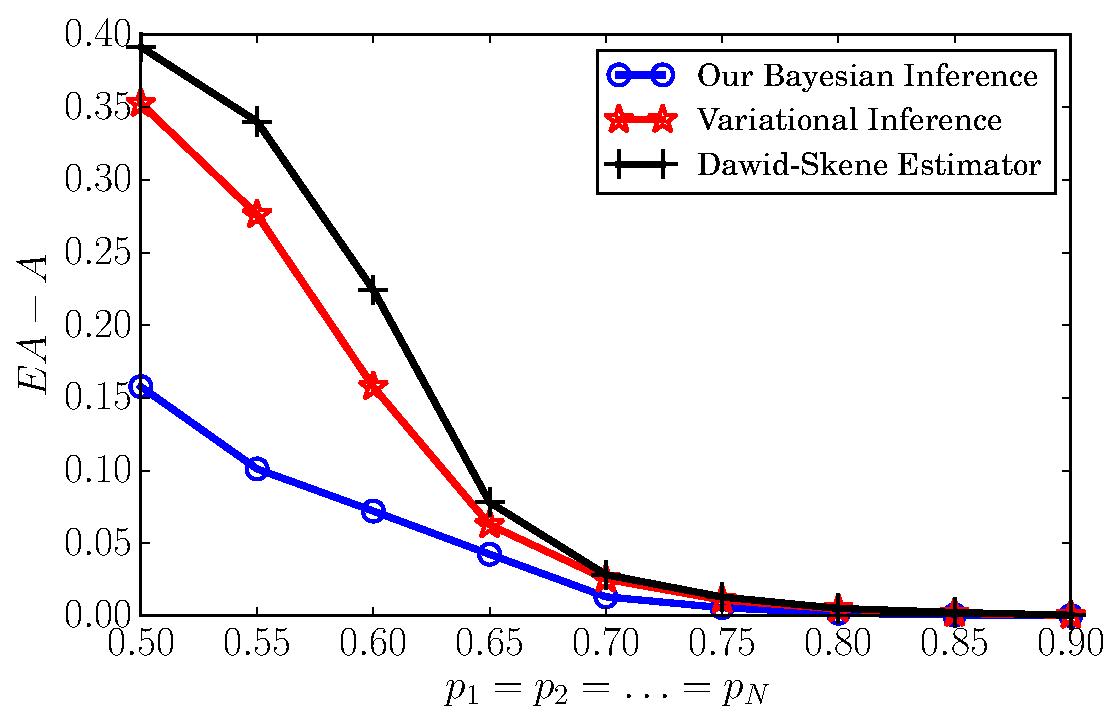
\includegraphics[width=\textwidth]{image/EXPC1}
        \caption{\label{BIM1}}
    \end{subfigure}
    ~
    \begin{subfigure}[t]{0.24\textwidth}
        \centering
        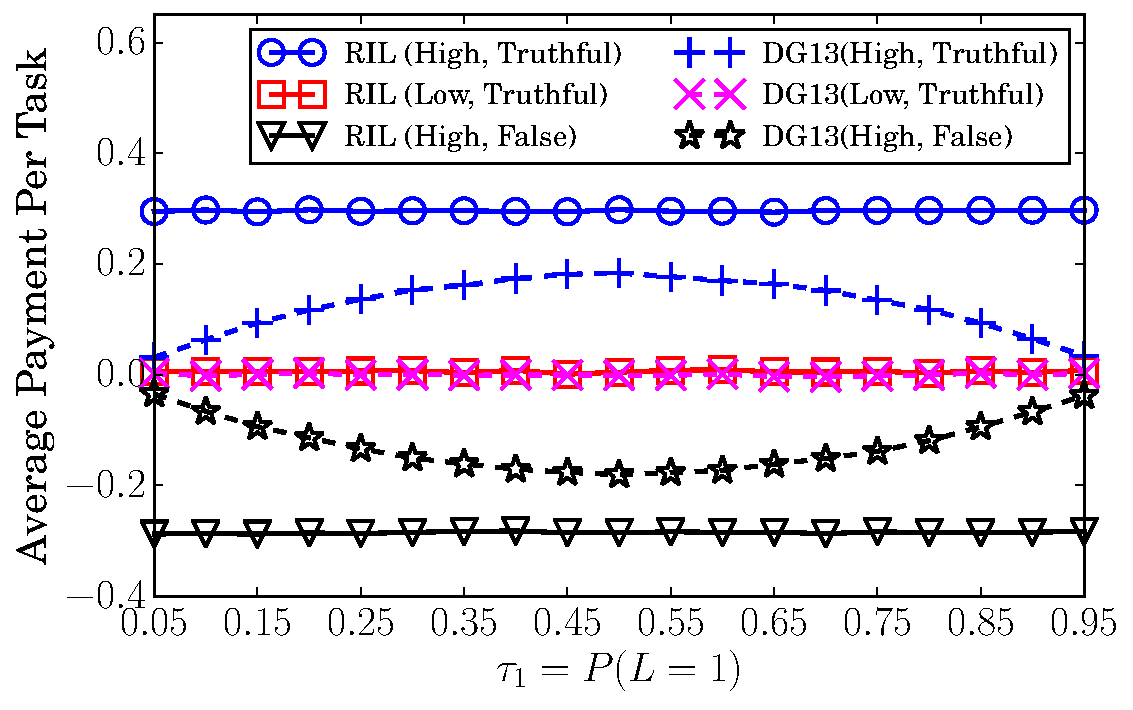
\includegraphics[width=\textwidth]{image/BPP1}
        \caption{\label{BIM2}}
    \end{subfigure}%
    ~
    \begin{subfigure}[t]{0.24\textwidth}
        \centering
        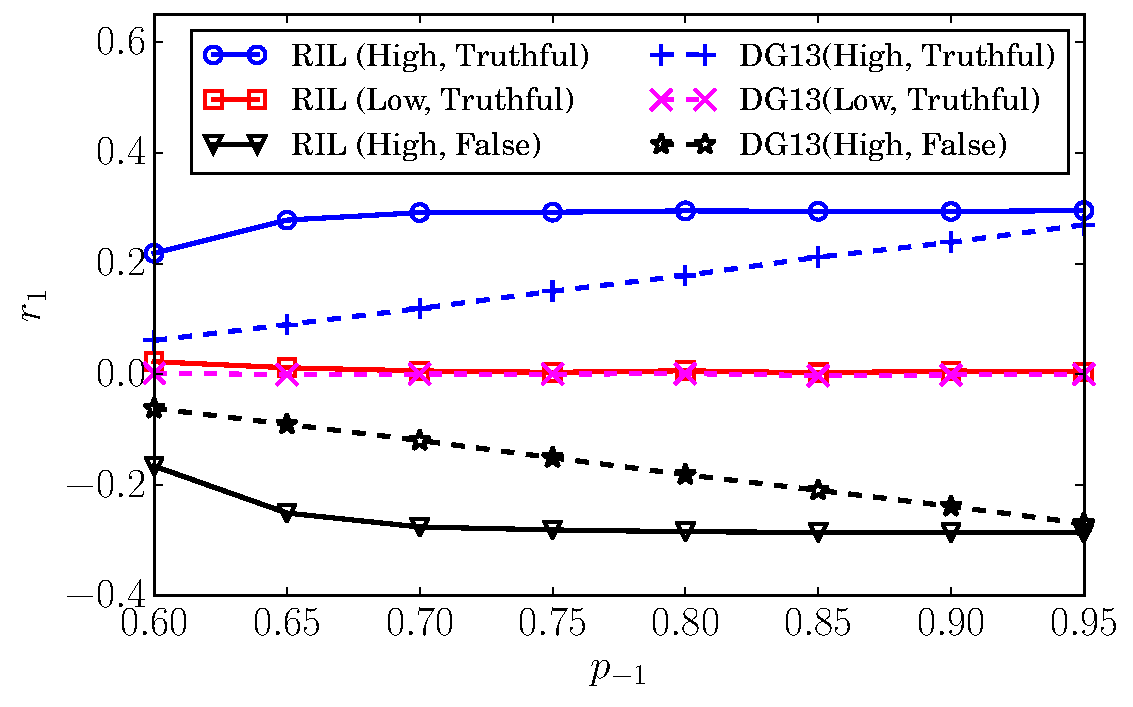
\includegraphics[width=\textwidth]{image/BPP2}
        \caption{\label{BIM3}}
    \end{subfigure}
        ~
    \begin{subfigure}[t]{0.24\textwidth}
        \centering
        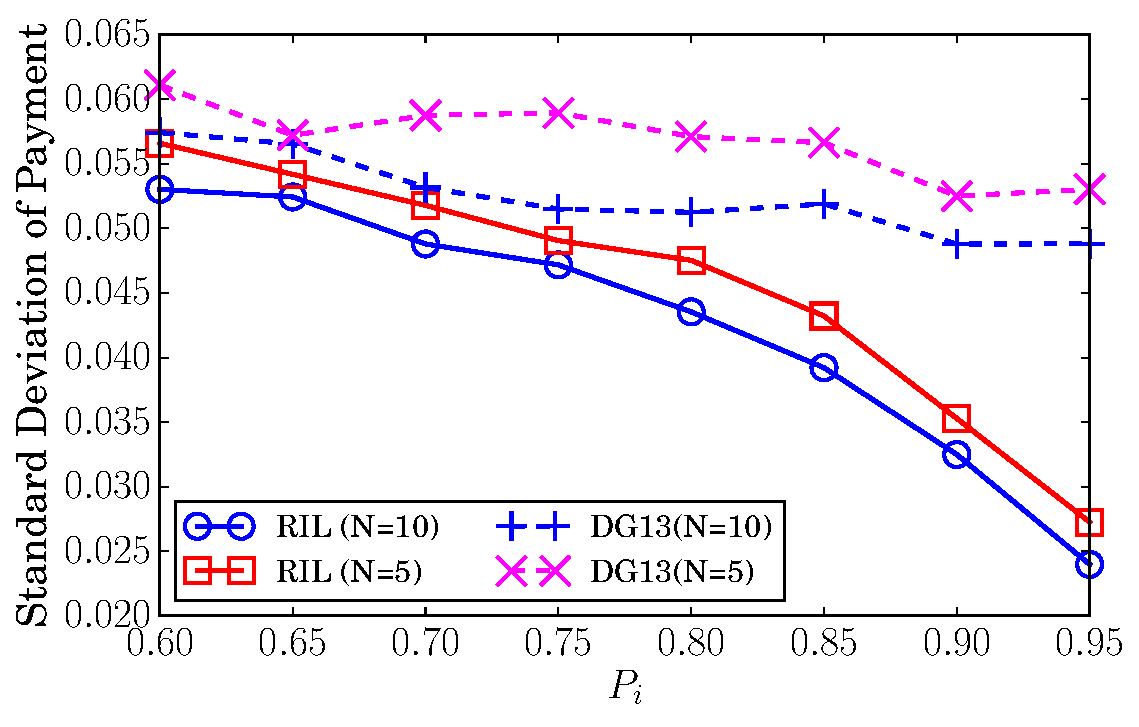
\includegraphics[width=\textwidth]{image/BPP3}
        \caption{\label{BIM4}}
    \end{subfigure}
    \vspace*{-3mm}
    \caption{\label{BIM}Empirical analysis on our one-step Bayesian incentive mechanism (BIM) (a) the inference bias (b) the reward variation as the distribution of true labels (c) the reward variation as the score of other workers (d) the standard variance of the reward for worker $1$}
\end{figure*}

\section{Empirical Experiments}
In this section, we conduct experiments on our Bayesian incentive mechanism at first to verify its advantages to lower the inference bias and improve the fairness and stability of the rewards for workers.
Then, to verify the advantage of our reinforcement incentive mechanism to boost the utility of the data requester, we empirically test our mechanism by using three representative worker models, including fully rational, bounded rational and self-learning agents.

\subsection{Bayesian incentive mechanism experiments}
In the literature of crowdsourcing, the Dawid-Skene estimator is the most popular method used to infer the true labels~\cite{dawid1979maximum,raykar2010learning}.
The variational inference estimator, which has the similar Bayesian model to our inference algorithm, is also widely-adopted in the existing studies of crowdsourcing~\cite{liu2012variational,chen2015statistical}.
To compare different estimators, we set $M=100$ and $N=10$ in Figure~\ref{BIM1}. Also, we let the score of all workers be equal, namely $p_1= \ldots=p_N$, and increase the value of $p_i$ from $0.5$ to $0.9$. Meanwhile, we set the true label distribution as the uniform distribution, namely $\tau_1=\tau_2=0.5$. For a given $p_i$, we firstly generate the true labels and then the labels of all workers both by the Bernoulli distribution. For each value of $p_i$, we run the experiments for $1000$ rounds. To show the bias of inference, we calculate the average value differences between the posterior expected accuracy $\mathbb{E}A$ and the real accuracy $A$. From the figure, we can find that, when workers can provide not-so-bad labels ($p_i>0.75$), both the two above estimators and our inference algorithm have very small bias, which agrees with the good performance of these estimators in the literature~\cite{raykar2010learning,liu2012variational}. However, if workers can only provide low-quality labels, the bias of the Dawid-Skene and variational inference estimators will become unacceptable, because the difference can be larger than $0.3$ while both $\mathbb{E}A$ and $A$ belong to $[0.5,1.0]$. In this case, we cannot use $\mathbb{E}A$ to calculate the utility of the data requester as Equation~\ref{utility}. By contrast, the bias of our Bayesian inference algorithm is much smaller, which is the foundation of our reinforcement incentive mechanism.


In Figures~\ref{BIM}b-d, we focus on $r_1$, namely, the per-task-reward received by worker $1$. Here, DG13~\cite{dasgupta2013crowdsourced,liu2017sequential}, which is the state-of-the-art incentive mechanism for binary labels, is employed as the benchmark.
DG13 decides the reward for a worker by comparing his labels with the labels provided by another randomly selected worker.
By elaborately designing the reward rules, it can also ensure reporting truthfully and exert high efforts to be a Nash equilibrium for all workers.
In all these experiments, we set $p_H=0.8$, $p_L=0.5$, and keep the other settings the same as those in Figure~\ref{BIM1}.

In Figure~\ref{BIM2}, we let $p_{-1}=p_H$, where the subscript $-1$ denotes all the workers except for worker $1$.
We change the distribution of true labels by increasing $\tau_1$ from $0.05$ to $0.95$ and compare the average values of $r_1$ corresponding to the different strategies of worker $1$.
In Figure~\ref{BIM3}, we fix the distribution of true labels to be the uniform distribution, namely, $\tau_1=\tau_2=0.5$, and increase $p_{-1}$ from $0.6$ to $0.95$.
From these two figures, we can find that the rewards provided by our mechanism are almost not affected by the variation of the distribution of true labels and the strategies of the other workers.
This observation reveals that $\mathbb{E}\tilde{p}_1$ converges to $p_1$ in most cases.
The only exception is $p_{-1}<0.7$ in Figure~\ref{BIM3} where the low-quality labels will lead to a remarkable bias of inference.
Even in this case, worker $1$ can only get the maximal reward when $p_1=p_H$, which shows the attracting ability of our mechanism to induce truthful reports and high efforts.
By contrast, $r_1$ in DG13 is severely affected by the distribution of true labels and the strategies of other workers.
For example, in Figure~\ref{BIM3}, if the other workers lower their efforts, the reward received by worker $1$ will also decrease, although worker $1$ never changes his strategies.
Thereby, for worker $1$, our Bayesian incentive mechanism is much fairer than DG13.

In Figure~\ref{BIM4}, we set $\tau_1=\tau_2=0.5$ and $p_{-1}=p_H$. We change worker $1$'s strategies by increasing $p_1$ from $0.6$ to $0.95$. Under these settings, the average values of $r_1$ corresponding to our mechanism and DG13 both can reflect the variation of $p_1$ very well. Thus, we focus on the standard variance comparison of $r_i$ in Figure~\ref{BIM4}.
If the variance is very large, the reward received by worker $1$ when $p_1=p_H$ may become lower than the reward when $p_1<p_H$.
If this case happens, it will significantly discourage worker $1$.
For example, in Figure~\ref{BIM2}, when $\tau_1=0.05$, for DG13, the difference between $r_1(p_1=p_H)$ and $r_1(p_1=0.5)$ is around $0.06$.
On the other hand, from Figure~\ref{BIM4}, the standard variance of $r_1$ is around $0.052$, which means there is a quite high probability for $r_1(p_1=p_H)<r_1(p_1=0.5)$.
From Figure~\ref{BIM4}, we can find that our Bayesian incentive mechanism has a lower variance than DG13.
If we take the fairness of our mechanism into consideration, we can conclude that our mechanism is more stable than DG13 in inducing truthful reports and high efforts from workers.


%\begin{equation}
%P(L(j)=1)=\tau_1{\prod}_{k\neq i}p_H^{\delta_{kj1}}(1-p_H)^{\delta_{kj2}}
%\end{equation}
%where $\lambda_0=\log(\tau_1/\tau_2)$ and $\lambda_i=\log(p_i/\bar{p}_i)$. For worker $i$, we assume that all other workers report truthfully and exert high efforts. Suppose the real true label is $1$. In order to ensure $\mathbb{E}[m/M]$ to approach $0$, the probability ratio in Equation~\ref{Ratio} must be positive with almost $1.0$ probability. Thus, we can directly discard the absolute operation in Equation~\ref{vot} and calculate the expected value of task $j$ as
%\begin{equation}
%\mathbb{E}_1v(j)\approx \lambda_0+(N-1)(2p_H-1)\lambda_H+(2p_i-1)\lambda_i.
%\end{equation}
%Similarly, if the real true label is $2$, then
%\begin{equation}
%\mathbb{E}_2v(j)\approx -\lambda_0+(N-1)(2p_H-1)\lambda_H+(2p_i-1)\lambda_i.
%\end{equation}
%Thus, the average task value $v$ satisfies
%\begin{equation}
%\begin{split}
%&\mathbb{E}v = \tau_1 \mathbb{E}_1v(j) + \tau_2\mathbb{E}_2v(j)\\
%&=(2\tau_1-1)\lambda_0+(N-1)(2p_H-1)\lambda_H+(2p_i-1)\lambda_i.
%\end{split}
%\end{equation}
%
%Suppose the true label is $1$.
%\begin{equation}
%x= \log\frac{P(L=1)}{P(L=2)}=g+\sum_{i=1}^{N}f(x_i,y_i,w_i,z_i)
%\end{equation}
%\noindent where $g=g_1-g_2$, and 
%\begin{equation*}
%g_1=\log(s_1+t_2+1)\;,\;g_2=\log(s_2+t_1+1).
%\end{equation*}
%Omitting the subscript in $f$, we can have $f=f_1-f_2$ with probability $p$ and $f=f_2-f_1$ with probability $1-p$. Here,
%\begin{equation*}
%f_1=\log(x+z+2)\;,\;f_2=\log(w+y+1).
%\end{equation*}
%Thus, we can have
%\begin{equation}
%\mathbb{E}g = \mathbb{E}g_1-\mathbb{E}g_2 \;,\;
%\mathbb{E}f = (2p-1)(\mathbb{E}f_1-\mathbb{E}f_2).
%\end{equation}
%From the previous proof, we know that $P(m)$ is very small when $m>>1$. Thus, we mainly focus on the region where $m$ is relatively small. For a given small $m$,
%\begin{equation}
%\mathbb{E}_{s_1, t_2}g_1\approx \mathbb{E}_{t_2}\log(np+t_2+1)
%\end{equation}
%\begin{equation}
%\log(np+t_2+1) = \log(np+1)+\sum_{i=1}^{\infty}(-1)^{i-1}q^i
%\end{equation}
%\begin{equation}
%q = \frac{t_2}{np+1}\Rightarrow 0\leq q^{i} \leq c^{i}\cdot \left(\frac{m}{M}\right)^i\leq c^{i}\frac{m}{M}
%\end{equation}
%Then,
%\begin{equation}
%\mathbb{E}g_1 \approx \mathbb{E}_{m}\log(1+Mp-mp)
%\end{equation}
%\begin{equation}
%\log(1+Mp-mp)\approx\log(1+Mp)+\sum_{i=1}^{\infty}(-1)^{i}\left(\frac{m}{M}\right)^i
%\end{equation}
%Using the similar way of approximation for the computation of $\mathbb{E}g_2$, $\mathbb{E}f_1$ and $\mathbb{E}f_2$, we can have
%\begin{equation}
%\begin{split}
%\mathbb{E}g_1\approx \log(Mp)\;,\;\mathbb{E}g_2\approx \log(M(1-p))\\
%\mathbb{E}f_1\approx \log(Mp)\;,\;\mathbb{E}f_2\approx \log(M(1-p))
%\end{split}
%\end{equation}
%Thus, if all workers exert high efforts and report truthfully,
%\begin{equation}
%    \mathbb{E}x \approx \log\lambda_0 + {\sum}_{i=1}^{N}\log\lambda_{i,H}
%\end{equation}
%If the true label is $2$, then
%\begin{equation}
%    \mathbb{E}x \approx \log\lambda_0 - {\sum}_{i=1}^{N}\log\lambda_{i,H}
%\end{equation}
%Thereby,
%\begin{equation}
%    \mathbb{E}|x|\approx (2p_0-1)\log\lambda_0+ {\sum}_{i=1}^{N}\log\lambda_{i,H}
%\end{equation}
%When, for example, worker $1$ deviate from the desired equilibrium strategy, the non-equilibrium state correspond to
%\begin{equation}
%    \mathbb{E}|x'|\approx (2p_0-1)\log\lambda_0+ \log\lambda_{1}+{\sum}_{i=2}^{N}\log\lambda_{i,H}
%\end{equation}
%The minimal value of $\mathbb{E}|x'|$ is reached when worker $1$ exert high efforts and report falsely, namely $\log\lambda_{i}=-\log\lambda_{i,H}$.
%Thus, the maximal reward increment brought by worker $1$'s strategy switch is
%\begin{equation}
%    V_1 = F(\mathbb{E}x)-F(\mathbb{E}x') \approx 2\log\lambda_{1,H}\cdot \left.\frac{\mathrm{d}F}{\mathrm{d}x}\right|_{x=x_H}
%\end{equation}
%Since $p_0$ is difficult to estimate, we define the upper bound of the value increment as
%\begin{equation}
%    V = 2\max_{i}\log\lambda_{i,H} \cdot  \max_{x\in [x_H, \infty)}\frac{\mathrm{d}F}{\mathrm{d}x} 
%\end{equation}
%where $x_H= \log\lambda_0 + {\sum}_{i=1}^{N}\log\lambda_{i,H}$.
%Considering the discounted reward calculation in reinforcement learning, we can know the maximum value difference can be created by the manipulation of any worker is $(1-\rho)^{-1}V$. Meanwhile, if the reinforcement part increases the scaling factor by $\delta$ to obtain the reward increment, we need to pay more than $\sum_{i=1}^{N}M\delta (p_{i,H}-0.5)$. Thus, if we want to prevent the reinforcement learning module from the adversarial manipulation, the minimal gap $\delta$ between to two available scaling factors should satisfy
%\begin{equation}
%    \sum_{i=1}^{N}M\delta (p_{i,H}-0.5) > V.
%\end{equation}